\section{Dodatek}

\subsection{Przebieg poświęcenia wody}
\label{sec:woda}
\begin{enumerate}
      \item \textit{Dominus Vobiscum} i Oracja 0. (przed wejściem)
            \smallfont{(złożone ręce)}
      \item \textit{Dominus Vobiscum} i Oracja 1. \smallfont{(złożone ręce)}
      \item Prefacja do słów \textit{Sumat unigeniti tui gratiam de Spiritu
                  Sancto}
      \item \ii~ kreśli znak krzyża
            \textcolor{red}{\raisebox{-1mm}{\scalebox{1.5}{\ding{64}}}} na
            wodzie
      \item Wyciera ręce
      \item Kontynuuje modlitwę
      \item Na \textit{Sit haec} kładzie rękę na powierzchni wody
      \item Wyciera rękę
      \item Kreśli znaki krzyża
            \textcolor{red}{\raisebox{-1mm}{\scalebox{1.5}{\ding{64}}}}
            nad wodą na słowa \textit{Per Deum vivum \dots}
            \vspace*{-11pt}
      \item Wylewa wodę na cztery strony świata po słowach \textit{... super te
                  ferebatur} ~~~
            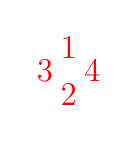
\begin{tikzpicture}[scale=0.3, baseline=-1mm, thick]
                  \draw[color=red] (10mm,0) node {\large 4};
                  \draw[color=red] (-10mm,0) node {\large 3};
                  \draw[color=red] (0,10mm) node {\large 1};
                  \draw[color=red] (0,-10mm) node {\large 2};
            \end{tikzpicture}
            \vspace*{-7pt}
      \item Kreśli znak krzyża nad wodą na \textit{Benedico te}
      \item Po zmianie głosu na \textit{recto tono} na słowa \textit{tu benignus
                  aspira} trzy razy dmucha do wody na kształt krzyża
      \item W tym czasie \cc1 podaje Paschał
      \item Na słowa \textit{Descendad in hanc} trzy razy wkłada Paschał do wody
            i śpiewa \footnote{Wkłada Paschał coraz głębiej}
      \item \ii~ trzy razy dmucha do wody w kształcie litery
            \textcolor{red}{\raisebox{-1mm}{\Large ${\Psi}$}} i kontynuuje
            \textit{Totamque ... effectu}
      \item Wyciągamy Paschał z wody i kończymy święcenie wody (\textit{... per
                  ignem.})
      \item Po \textit{Amen} nabiera się wody do pokropienia
      \item Pokropienie i \textit{Com przyrzekł Bogu \dots}
      \item Następnie \cc1 przynosi do chrzcielnicy tackę z olejami świętymi i
            wręcza \ii~ (z pocałunkiem) odpowiednie ampułki. \ii, wypowiadając
            słowa przepisane w księdze po kolei:
            \begin{itemize}
                  \item wlewa olej katechumenów
                  \item wlewa krzyżmo
                  \item wlewa oba
            \end{itemize}
      \item Następnie miesza wodę ręką lub przy pomocy łyżeczki \footnote{W
                  razie potrzeby myje i wyciera ręce; wykorzystuje sól, watę i
                  miękisz chleba, które później należy spalić. Wodę z tej
                  ablucji wlewa się do sacrarium.}
\end{enumerate}

\subsection{Obrzędy wstępne chrztu dorosłego}
\label{sec:chrzest}
\begin{itemize}
      \item Podejście do przedsionka
      \item Dialog (\textit{jak ci na imię ...})
      \item 3 $\times$ dmucha w twarz, mówi, dmuch w kształcie \krzyz, modlitwa
      \item Modlitwa i \krzyz~ na czole potem \krzyz~ na piersi
      \item Modlitwa i \krzyz\krzyz~ na uszach, \krzyz\krzyz~ na oczach,
            \krzyz\krzyz~ na nozdrzach, \krzyz~ na ustach, \krzyz~ na piersi i
            \krzyz~ na plecach
      \item Duży \krzyz~ nad całym katechumenem
      \item Sól w usta i modlitwa
      \item Katechumen klęka, mówi \textit{Ojcze nasz} i wstaje
      \item Ojciec chrzestny kreśli \krzyz~ na czole katechumena, potem robi to
            \ii
      \item \ii~ kładzie ręce na głowie i czyta modlitwy
      \item Katechumen klęka, mówi \textit{Ojcze nasz} i wstaje
      \item Ojciec chrzestny kreśli \krzyz~ na czole katechumena, potem robi to
            \ii
      \item \ii~ kładzie ręce na głowie i czyta modlitwy
      \item Katechumen klęka, mówi \textit{Ojcze nasz} i wstaje
      \item Ojciec chrzestny kreśli \krzyz~ na czole katechumena, potem robi to
            \ii
      \item \ii~ kładzie ręce na głowie i czyta modlitwy
      \item Katechumen łapie stułę w rękę i wchodzą do kościoła (modlitwa)
      \item Padniecię na twarz i pocałunek podłogi
      \item Znowu łapie stułę i idąc dalej mówią \textit{Wierzę w Boga, Ojcze
                  Nasz} \footnote{idziemy od kruchty do ołtarza NOM środkiem,
                  potem w lewo i do baptysterium}
      \item Ręka nad głowę i egzorcyzm
      \item Ślina na palec i dotknięcie uszu i nosa
      \item Dialog (\textit{jak ci na imię?, odrzekasz się?})
      \item Palec w olej katechumenów i \krzyz~ na piersi i \krzyz~ ponad
            łopatkami
      \item Wytarcie oleju
\end{itemize}

\subsection{Bierzmowanie}
\label{sec:bierz}
\begin{enumerate}
      \item księgę trzyma \ss, a \cc1 stoi z boku z mikrofonem, \cc2 przy
            kredencji
      \item \ii~ zwraca się do kandydatów \textit{Spiritus
                  Sanctus superveniat\dots Amen.}
      \item \ii~ żegna się mówiąc \textit{Adjutorium nostrum...}, potem krótki
            dialog
      \item \ii~ wyciąga ręce nad kandydatami i mówi
            \textit{Oremus. Omnipotens sempiterne Deus,\dots}
      \item Bierzmowany klęka przed \ii. Świadek kładzie rękę na
            prawym ramieniu bierzmowanego.
      \item \cc2 podchodzi do \dd~ z Krzyżmem Świętem
      \item \ii~ kładzie prawą rękę na głowie bierzmowanego i palcem umoczonym w
            Krzyżmie Świętym robi znak krzyż a na czole, mówiąc \textit{Signo te
                  signo\dots}
      \item \ii~ uderza lekko w policzek bierzmowanego, mówiąc \textit{Pax tecum}
      \item \cc2 z ojcem chrzestnym zakładają opaskę na czoło bierzmowanego
      \item Bierzmowany wraca na swoje wcześniejsze miejsce i klęczy
      \item Gdy \ii~ namaści wszystkich kandydatów, śpiewa się antyfonę
            \textit{Confirma hoc, Deus\dots}
      \item \cc2 odbiera Krzyżmo, i wraz z \aa3 podchodzi z solą, chlebem, wodą
            i ręcznikiem do wytarcia palców; później wraca do kredencji
      \item Powtarza się antyfonę, a następnie \ii~ zwrócony do ołtarza śpiewa
            \textit{Ostende nobis, Domine,\dots}
      \item Mówi \textit{Oremus. Deus, qui
                  Apostolis tuis\dots}
      \item \ii~ mówi \textit{Ecce sic benedicetur omnis homo, qui timet Dominum}
      \item Na końcu odwraca się do ludu i błogosławi bierzmowanych
            \textit{Bene} \textcolor{red}{\raisebox{-1mm}{\scalebox{1.5}{\ding{64}}}}
            \textit{dicat vos Dominus ex Sion\dots}
\end{enumerate}

\color{red}

\section{Poprawki}
\begin{itemize}
      \item dodać jeszcze jednego zakrystianina
      \item dłuższa litania i na zwyczajną melodię
      \item dodać \textit{Sicut servus} do ceremoniału \ii~(musi on być
            przeczytany przed wejściem do baptysterium)
      \item obrzędy wstępne nie muszą się odbywać całe na raz -- można co
            tydzien robić kolejny etap wprowadzający (całe obrzędy wstępne
            trwają 30 min)
\end{itemize}